% !TEX root =  ../main.tex

\section{Preliminaries}\label{sec:preliminaries}


A \emph{distribution} over a finite set $X$ is a function $\mu\colon X\rightarrow [0,1]$
where $\sum_{x\in X} \mu(x) = 1$. The set of distributions over $X$ is denoted by
$\Dist(X)$.

\subsubsection{Markov decision processes (MDPs)} 
An MDP is a tuple $\cM = (S,A,\imath,G,R,T)$ where 
$S$, $A$, and $G \subseteq S$ are finite sets of states, actions, and goal states, respectively,
$\imath \in S$ is an initial state, $R \colon S \rightarrow \Real$ is a reward function,
and $T\colon S{\times}A \pa \Dist(S)$ is a partial transition probability function.
For state $s\in S$ and action $a\in A$ we say that $a$ is \emph{enabled} in $s$ if
$T(s,a)$ is defined. We assume the set $\Act(s)$ of all enabled actions to be empty
in goal states $s\in G$ and non-empty in all other states.
For $(s,a,s')\in S{\times}A{\times}S$ we define $T(s,a,s')=T(s,a)(s')$ 
if $T(s,a)$ is defined and $T(s,a,s')=0$ otherwise.
The \emph{successors} of $s$ via $a$ are denoted by $\Post(s,a) = \{ s' \mid T(s,a,s')>0 \}$.
A \emph{run} of $\cM$ is a sequence $\pi = s_0a_0s_1a_1\dots s_n$
where $s_0=\imath$, $s_n \in S$, $(s_i,a_i)\in (S{\setminus}G)\times A$, 
and $s_{i+1}\in\Post(s_i,a_i)$ for $i= 0,\ldots,n{-}1$.
The set of all runs in $\cM$ is denoted by $\Runs(\cM)$.
The \emph{accumulated reward} of $\pi$ is defined by $R(\pi) = \sum_{i=0}^{n-1} R(s_i)$.



An \emph{interval MDP (IMDP)} is a tuple
$\cU=(S,A,\imath,G,R,\hat{T})$ where $S,A,\imath,G$, and $R$ are as 
for MDPs, and $\hat{T} \colon S {\times} A \pa \Intv(S)$ is an
\emph{interval transition function}. Here, $\Intv(S)$ denotes the set of interval functions
$\nu\colon S \ra \{ [a,b] \mid 0 < a \leq b \leq 1 \} \cup \{ [0,0] \}$ over $S$.
Note that $\Dist(S)\subseteq\Intv(S)$, i.e., every distribution over $S$ is also
an interval function. A distribution $\mu\in\Dist(S)$ is an \emph{instantiation} of 
$\nu\in\Intv(S)$ if $\mu(s)\in\nu(s)$ for all $s\in S$. 
We again say $a$ is enabled in $s$ if $\hat{T}(s,a)$ is defined and denote
the set of enabled actions in $s$ as $\Act(s)$, assumed to be non-empty for all $s\in (S\setminus G)$.
For each $s\in S$ and $a\in \Act(s)$ we denote by $T_s^a$ the set of 
all instantiations $t_s^a$ of $\hat{T}(s,a)$ and define $\Post(s,a)=\{s' \mid \underline{T}(s,a,s')>0\}$.
The MDP $\cM$ is an \emph{instantiation} of $\cU$ if 
$T(s,a)\in T_s^a$ for all $s\in S$, $a\in A$.
We denote by $[\cU]$ the set of all instantiations of $\cU$.
Note that as all instantiations of an IMDP $\cU$ share the same topology, 
the set of runs $\Runs(\cM)$ is the same for all instantiations $\cM\in[\cU]$.


The semantics of the MDP $\cM$ is given 
through \emph{strategies}, i.e., mappings $\sigma\colon S
\rightarrow \Dist(A)$ where $\sigma(s)(a)=0$ for all $a\not\in\Act(s)$. 
We call a run $\pi=s_0a_0s_1a_1\dots s_n$ 
in $\cM$ a \emph{$\sigma$-run} if $\sigma(s_i)(a_i)>0$ for all $i=0,\ldots,n{-}1$. 
The probability of $\pi$ is defined as $\Pr^\sigma(\pi) = \prod_{i=0}^{n-1} \sigma(s_i)(a_i)\cdot T(s_i,a_i,s_{i+1})$ if $\pi$ is a $\sigma$-run and $\Pr^\sigma(\pi)=0$ otherwise.
The probability of some $B\subseteq\Runs(\cM)$ w.r.t. strategy $\sigma$ is defined
by $\Pr^\sigma(B) = \sum_{\pi\in B} \Pr^\sigma(\pi)$.
If $\Pr^\sigma(B)=1$, then the \emph{expected (accumulated) reward} is defined
as $\Exp^\sigma(B) = \sum_{\pi\in B} \Pr^\sigma(\pi)\cdot R(\pi)$.
We call $\cM$ \emph{contracting} \cite{KalLN20} if $\Pr^\sigma(\lozenge G) = 1$ for all strategies $\sigma$, i.e., 
a goal state is almost surely reached for any strategy. 
The semantics of an IMDP $\cU$ is the set of its instantiations $[\cU]$. 
An IMDP $\cU$ is \emph{contracting} iff all MDPs in $[\cU]$ are contracting. 
Note that for IMDPs there is also a notion of an operational semantics that lifts strategies
to instantiations of transitions \cite{SenVisAgh06}. While different in its nature, our contributions 
of this paper can be easily extended also to the latter semantics.


\subsubsection{Value and quality functions}
A \emph{value function} $V_{\cM} \colon S \rightarrow \Real$ of MDP $\cM$ is the solution of the 
\emph{Bellman equations}~\cite{BerTsi91} given by $V_\cM(s)=R(s)$ for $s\in G$ and
\begin{center}
$V(s)\ =\
	R(s) + \max_{a\in \Act(s)} \sum_{s' \in S} V_\cM(s')\cdot T(s,a,s')$ \quad for \enskip $s\not\in G$.%& \text{else}
\end{center}
The \emph{quality} $Q_\cM\colon S\times A \pa \Real$ of $\cM$ is defined for all $s\in S$ and $a\in \Act(s)$ by
\begin{center}$
	Q_\cM(s,a)\ =\ R(s)\ + \sum\nolimits_{s' \in \Post(s,a)} V_\cM(s')\cdot T(s,a,s')
$\end{center}
Intuitively, the quality represents the value of choosing 
an action $a$ in state $s$ continuing with a reward-maximizing strategy.
For an IMDP $\cU$, the value function differs between instantiations, leading to
Bellman equations

\begin{center}
	$\underline{V}_\cU(s)\ =\  \min_{\cM\in [\cU]}{V_\cM(s)} \quad\quad
\overline{V}_\cU(s) =\max_{\cM\in [\cU]}{V_\cM(s)}$
\end{center}
for the lower and upper bounds on possible instantiations, respectively. 
These value functions are naturally lifted to quality functions for IMDPs.
We omit subscript $\cM$ or $\cU$ if clear from the context.
Further, we define the \emph{pessimistically optimal strategy}
$\underline{\sigma}$ for all $s\in (S\setminus G)$ as
$\underline{\sigma}(s)=\argmax_{a\in\Act(s)}\underline{Q}(s,a)$ and similarly the
\emph{optimistically optimal strategy} as
$\overline{\sigma}(s)=\argmax_{a\in\Act(s)}\overline{Q}(s,a)$.

\begin{figure}[t]
	\resizebox{\textwidth}{!}{\section{Proof-of-Concept Expert System for Software Protection}
\label{sec:workflow}

\label{sec:esp:kb}

Expert systems exist in cybersecurity since 1986 when Hoffman proposed one for the risk analysis of computer networks~\cite{hoffman1986risk}. From the initial intrusion detection systems~\cite{idesReq,audes} to  modern ones using AI~\cite{owensIDS}, expert systems have been used to automatically configure security controls~\cite{fwExpSys}, for post-incident network forensics~\cite{kimForensics,liaoForensics} and decision making.

The Expert System for Software Protection (\esp) is our \poc tool that implements a semi-automated \softprot risk analysis\footnote{In the ASPIRE project and in some cited papers, the ESP was called the ASPIRE Decision Support System (ADSS).}. Its complete code is available\footnote{\url{https://github.com/daniele-canavese/esp/}}, as well as a technical report on its inner workings~\cite{D5.11}, a user manual~\cite{D5.13}, and a demonstration video\footnote{\url{https://www.youtube.com/watch?v=pl9p5Nqsx_o}}.
%
The \esp is primarily implemented in Java as a set of Eclipse plug-ins with customized UI. 
It protects software written in C and needs source code access. 
The target users are software developers or \softprot consultants.
%The \esp has been designed to perform as many tasks as possible without human intervention. 
After the user manually annotates the assets in the source code, the \esp can generate what it considers optimally protected binaries and the corresponding security-server-side logic without human intervention.
As requested by the \softprot experts involved in the evaluation, a step-wise execution is also available where users can check and possibly override any information generated by the tool before executing the next step. 
\begin{figure}[t]
	\centering
    \includegraphics[width=6cm]{images/workflow}
	\caption{The \esp workflow.}
	\label{fig:workflow}
\end{figure}

% Also for the \esp, an \emph{asset} is a software component (\ie a variable or a code region) with some security requirement that must be safeguarded against attackers. % (\eg a cryptographic key must be kept confidential). 

% We will use the term \emph{solution} to denote an ordered sequence of protections (and their related configurations) that can be used to safeguard all the security properties of an application's assets. We are particularly interested in finding the \emph{golden solution}, that is the most secure solution that can be applied to protect a software application. Ultimately, the job of the \esp is to find the golden solution without any human intervention.


Figure~\ref{fig:workflow} depicts the high-level workflow, split into the four phases discussed in Section~\ref{sec:requirements}. %, namely, risk framing, risk assessment, risk mitigation, and risk monitoring.

All the data needed for the risk analysis process, starting from the \emph{risk framing} information and including all the data obtained during the other three phases, are modeled and stored in a \kb.
The used model and corresponding \kb structure are designed specifically to support the reasoning methods needed for a software risk analysis~\cite{reganoMeta}.
For example, it allows representing context information, like the attacker model and the {\softprot}s available to mitigate the risks, and information about the application to protect, including the assets and abstract representations of the application code collected through code analyses.  More details about these constructs and the model are presented in Section~\ref{sec:esp:risk_framing}.

Next, the \esp performs the \emph{risk assessment} phase, whose details are provided in Section~\ref{sec:esp:risk_assessment}. This phase enriches the data in the model. %
It infers the possible attacks against the assets and assesses the risks against each asset by estimating the complexity of executing those attacks. 
The risk is evaluated by considering the software's structure and the attacker model, \ie the skills an attacker is likely to have, and asset values as defined by the user during the risk framing. 
%   
The \esp's \emph{risk mitigation} phase, detailed in Section~\ref{sec:esp:risk_mitigation}, is also based on innovative methods. It uses \gls{ml} and optimization techniques to select the best \emph{solution}, i.e., the best sequence of {\softprot}s to be deployed and their configurations. It then automatically deploys it on the software to generate the protected application binaries.
If remote {\softprot}s are included in the selected solution, the deployment phase also generates the server-side logic to be executed on a trusted remote entity.

Finally, the \emph{risk monitoring} is performed. However, the \esp does not dynamically update the risk analysis process parameters. It only performs real-time integrity checking (as discussed in Section~\ref{sec:monitoring_relaesed}) depending on the methods implemented by the {\softprot}s used.


The \esp can also be used in two additional modes. It can be configured to propose a set of solutions that experts can manually edit to control the {\softprot} deployment fully. Moreover, it can be used to evaluate the effectiveness of solutions manually proposed by experts.



%%%%%%%%%%%%%%%%%%%%%%%%%%%%%%%%%%%%%%%%%
\subsection{Risk Framing in the ESP}
\label{sec:esp:risk_framing}

% MISSING\constructlab{30}

This tasks' purpose is to initialize all the constructs and their relations as needed for risk analysis, and to store them into a model formally defined in~\cite{reganoMeta} and named the \kb. It covers half of the models (\modellab{1}, \modellab{4}, \modellab{5}) highlighted in Section~\ref{sec:requirements}. Figure~\ref{fig:metaModel} presents the core classes, which will be discussed in the next sections. The \kb is instantiated as an OWL~2 ontology~\cite{owl2}.

The \emph{risk framing} starts with the preparation of the \kb with \emph{generic a-priori information}. This includes the core concepts and data not related to the specific application to be protected but relevant to framing the risk analysis process.
A priori information includes the assets types (\constructlab{1}, \constructlab{2}); the supported security requirements (\constructlab{8}, \constructlab{9}, \constructlab{12}, \constructlab{13},  \constructlab{14}); all the known attack steps and their characterization (\constructlab{4}, \constructlab{17}, \constructlab{18}, \constructlab{20}, \constructlab{21}, \constructlab{22}); the available {\softprot}s and their composability (\constructlab{24}, \constructlab{26}, \constructlab{27}, \constructlab{28}, \constructlab{29}); and the necessary constructs to evaluate risks and mitigations (\constructlab{23}, \constructlab{25}, \constructlab{30}, \constructlab{31}, \constructlab{32}, \constructlab{33}) that were discussed in Section~\ref{sec:framing}.
The user can also set preferences and analysis parameters (\constructlab{38}, \constructlab{44}), including hard and soft constraints and SDLC requirements (\constructlab{34}, \constructlab{36}), as well as the {\softprot}s to consider and the kinds of attacks to counter.

The \esp then performs a \emph{source code analysis} (\methodlab{2}) that populates the \kb with \emph{a-priori analysis-specific information} using the Eclipse C Development Toolkit\footnote{\url{https://projects.eclipse.org/projects/tools.cdt}}.
The analysis collects all the \emph{application parts}, \ie the variables, functions, and code regions. It determines additional information such as variables' data types and function signatures. It produces additional representations such as the call graph, which are useful for making decisions about the {\softprot}s to apply.


The \poc of the \esp supports confidentiality and integrity requirements. 
The user needs to annotate the source code with custom pragma and attribute annotations~\cite{D5.11,D5.13} to formally identify the code's assets and to specify their security requirements (\methodlab{1}, \methodlab{5}). 
%
The ESP then uses the call graph to identify potential secondary assets. These are listed in the GUI where the user can manually select which ones are to be considered assets in the later phases, and with which security requirements (\methodlab{3}, \methodlab{4}). Using only a call graph as a model (\modellab{2}) to find potential secondary assets that need to be manually confirmed is overly simple, and hence definitely a topic of future research.
%

%





Together with a-priori information, the \kb model represents \emph{a-posteriori information}, \ie data inferred and stored during later workflow phases such as the inferred attacks and the solutions.

\begin{figure}[t]
	\centering
    \includegraphics[width=8cm]{images/metamodel.jpg}
% 	\includegraphics[width=0.99\linewidth]{images/kb.pdf}
	\caption{The top level of \esp meta-model to support modeling the relations between all relevant constructs.}
	\label{fig:metaModel}
\end{figure}


{
% \color{green!50!black} 

In addition, the \esp offers a GUI to edit the framing information, e.g., to mark additional assets, characterize the attacker, and choose {\softprot}s. The GUI also allows importing and exporting risk framing data as XML or OWL files (\methodlab{6}).
%
This feature was appreciated during the validation as it allows augmenting the analysis with information that may be missed by the automatic but as of yet incomplete process, like the secondary assets that might be linked into a protected program as part of certain {\softprot}s.}


%During this phase, the \esp parses the source code for the annotations that mark the assets and their  security requirements in the source code. Annotations are source code constructs manually added by the developers via ad-hoc C pragmas and GCC-like variable attributes. \dcnote{Should we put an annotation example here? Not sure.}  \abnote{add cite for annotations}
%Moreover, primary and secondary assets can also be selected from the list of discovered application parts from an \esp GUI.  \bdsnote{And they can also be added to the knowledge base through JSON or XML files, not? I think this is important for when code injected by the tool chain after this phase needs to be protected as well.} \dcnote{Yes, you can! The knowledge base is an OWL2 ontology, which is an XML file. You can edit it as you wish, also using an OWL editor like protege (https://protege.stanford.edu).}


\subsection{Risk Assessment in the ESP}
\label{sec:esp:risk_assessment}

The risk assessment implements several methods to estimate the actual threats and risks. In the \emph{threat analysis}, the \esp uses backward reasoning methods (\methodlab{7}) to identify the attacks (\constructlab{39}) that can breach the primary assets' security requirements, and stores them in the \kb~\cite{reganoProlog}. 
This stage is roughly equivalent to the ISO27k ``identify risk'' step as discussed in sections~\ref{sec:standardizedRisk} and~\ref{sec:assessment}. 

The identified attacks are represented as a set (\modellab{6}) of \emph{attack paths} (\constructlab{3}). % \conceptlab{3}.
These are ordered sequences of atomic attacker tasks called \emph{attack steps} (\constructlab{4}).  %\conceptlab{4}. 
Attack paths are equivalent to attack graphs~\cite{attack_graphs} and can serve to simulate attacks with Petri Nets~\cite{petri_nets_attacks}. 
The attack steps that populate our \poc\ \kb originate from a study and taxonomy by Ceccato\etal~\cite{ceccatoTaxonomy,emse2019} and from data from industrial \softprot experts who participated in the ASPIRE project.

The attack paths are built via backward chaining (\methodlab{7}) as proposed in earlier work~\cite{basileOTP,reganoProlog} and implemented with SWI-Prolog~\cite{SWI-Prolog}.
%\footnote{\url{https://www.swi-prolog.org/}}.
An attack step can be executed if its premises are satisfied. It produces the results of its successful execution as conclusions.
The chaining starts with steps that allow reaching an attacker's final goal (the breach of a primary requirement) and stops at steps without any premise.
The search algorithm builds a proof tree with increasing depth and width, with exponential complexity. The \esp hence implements basic yet aggressive search space pruning to build an attack catalogue, e.g., by considering a maximum length for the inferred attack paths~\cite{ReganoPhd}. The proof tree models the actual threats (\modellab{6}). Its nodes can be seen as the exploited attack vectors (\constructlab{42}), of which the leaves form the identified attack surface (\constructlab{41}).

The \esp performs the \emph{threat impact evaluation} (\methodlab{8}) and \emph{risk prioritization} (\methodlab{9}) by assigning a \emph{risk index} (\constructlab{40}) to each identified attack path. Every attack step in the \kb is associated with multiple attributes, including the \emph{complexity} to mount it, the minimum \emph{skills} required, the availability of support \emph{tools} and their \emph{usability}.  %\conceptlab{20-23}.  
Additional attributes can be associated with entities trivially. 
Each attribute assumes a numeric value in a five-valued range.
For assessing the actual risks, the values of complexity metrics and software features (\constructlab{45}) computed on the involved assets (\methodlab{10}) with the available analysis tools (\constructlab{44}) are used as modifiers on the attributes (\constructlab{22}). 
For instance, an attack step labelled as medium complexity can be downgraded to lower complexity if the asset to compromise has a cyclomatic complexity below some threshold.

The risk index of an attack path is obtained by aggregating the modified attributes of its steps into a single value (\methodlab{8}). Our \poc is rather simple. Per attack step, it first aggregates all the step's modified attributes into a single attack step risk index. The attack path risk index is then computed by multiplying its steps' indices. Other aggregation functions are supported, such as summing the steps' indices, selecting maxima, and more complex features can easily be incorporated, like making the attack path risk index depend on how many different expert tools are required.

The report (\methodlab{13}) presenting the attack paths and the computed risk indices was welcomed by security experts (as will be discussed in more detail in Section~\ref{sec:esp:results}), amongst others because they serve as a starting point for evaluating the weaknesses of an application before more manual risk mitigation. Experts were interested in refining the identified, most risky paths into more concrete sequences of attack operations, and in some cases, they would have manually updated the risk indices.
In our \poc, the attack steps are coarse-grained, such as ``locate the variable using dynamic analysis'' and ``modify the variable statically''.
This is an important limitation. As Section~\ref{sec:identification_threats} discusses, understanding how much refinement is needed is an open research question.




%%%%%%%%%%%%%%%%%%%%%%%%%%%%%%%%%%%%%%%%%%%%%%%%%%%%%%%%%%
\subsection{Risk Mitigation in the ESP}
\label{sec:esp:risk_mitigation}


Before presenting the ESP's risk mitigation process \methodlab{16}, we introduce more precise constructs. %\constructlab{24}
%
In the ESP, a \emph{\softprot} is a specific implementation of a \softprot technique by a specific \softprot tool.
For instance, control flow flattening~\cite{wangFlatteningTechReport} as applied by Diablo in the \actc and by Tigress are considered distinct {\softprot}s~\cite{tigress,diablo}.\footnote{\url{https://github.com/aspire-fp7/actc} and \url{https://tigress.wtf/}}
%
A \emph{protection instance} (PI) is a concrete configuration of a \softprot technique.
The \esp can use the PI to drive the \softprot tool to apply a {\softprot} technique on a chosen application part.
Depending on the available parameters, multiple PIs can be defined for the same {\softprot}. 
%, but only the most significant ones are selected to limit the number of instances to consider during the optimization. For example, Diablo takes as input a parameter that specifies the percentage of the target code that must be obfuscated. Meaningful PIs are obtained using 10\%, 20\%, 50\%, however, not 21\% and \22\%.
%    
An \emph{applied PI} is the association of a PI with an application part, which states that the PI has been selected to be applied to the part. %\bdsnote{Includes configuration parameters?} %\abnote{I don't like DPI but...}\dcnote{In the original ADSS I called them APIs (applied PIs).}
%    
A \emph{candidate solution} is a sequence of applied PIs. It is ordered because of composability and layering requirements and benefits (\constructlab{27}).


The \esp first searches for \emph{suitable {\softprot}s}. These are {\softprot}s that impact attributes of the listed attack steps (\methodlab{19}). For example, they are able to defer an attack step.
% A {\softprot} is deemeed suitable to defer an attack path if it is able to defer at least one attack step on the path.
Each PI is associated with a formula that alters these attributes for each attack step. 
After the application of a {\softprot}, the risk index of the attack steps and paths are re-assessed. 

The formulas also consider complexity metrics (\constructlab{25}) computed on the protected assets' code. This way, the ESP incorporates Collberg's prescription of \emph{potency}~\cite{collberg1997taxonomy} (\constructlab{30}) as a measure of the additional effort that attackers have to invest on protected code. 
%that are best able to defer the previously found attack paths.
The parameters to be used in the formulas for evaluating the impact of SPs on attack steps are stored in the \kb. 
They are based on a survey among the developers of all {\softprot}s integrated into the ASPIRE \softprot tool flow~\cite{D5.11}, whom we asked to score the impact of their {\softprot}s on a range of attack activities in terms of concrete impacts. 
These include the impact on human comprehension difficulty by increasing code complexity, the impact of moving relevant code fragments from the client-side software to a secure server not under the control of an attacker~\cite{renewability,codeMobility,viticchie2016reactive}, the impact on the difficulty of tampering through anti-tampering techniques with different reaction mechanisms and monitoring capabilities~\cite{viticchie2016reactive}, and the impact of preventive {\softprot}s such as anti-debugging~\cite{circulardebugging,diabloSelfDebugging}. 
The survey results were complemented with expert feedback and validated in pen test experiments~\cite{ceccatoTaxonomy,emse2019}.

Additional modifiers are activated when specific combinations of PIs are applied on the same application part. They model the impact of layered {\softprot}s (\constructlab{28}) when recomputing the risk indices and synergies between {\softprot}s. The existence of synergies (\constructlab{29}) was part of the mentioned survey. 

Candidate solutions must also meet cost and overhead constraints (\constructlab{33}). 
%\conceptlab{x}. 
Our \poc filters candidate {\softprot}s using five overhead criteria: client and server execution time overheads, client and server memory overheads, and network traffic overhead. 

Finally, the \emph{{\softprot} index} associated with a candidate solution is computed based on the recomputed risk indices of all discovered attack paths against all assets, weighted by the importance associated with each asset. The {\softprot} index is the ESP's instantiation of residual risk (\constructlab{47}).


\subsubsection{Asset Protection Optimization}
\label{sec:esp:risk_mitigation:optimization}
\label{sec:esp_optimization_approach}
The \esp finds the mitigations by building an optimization model that it solves with a game-theoretic approach (\methodlab{23}). The \esp tries to combine the suitable {\softprot}s to build the optimal layered  solutions, i.e., the candidate solution that maximizes the {\softprot} index and satisfies the constraints.

Computing the {\softprot} index by re-computing the risk index requires knowledge of the metrics on the protected application. As applying all candidate solutions would consume an infeasible amount of resources, we have built an \gls{ml} model to estimate the metrics delta after applying specific solutions without building the protected application~\cite{reganoMetric}. %\methodlab{26}. 
The ESP's ML model has been demonstrated to be accurate for predicting variations of up to three PIs applied on a single application part. With more {\softprot}s, however, the accuracy starts decreasing significantly. This issue seems to be solvable with larger data sets and more advanced \gls{ml} techniques.

The \esp uses the same predictors to estimate the overheads associated with candidate solutions. Per PI and kind of overhead, the \kb stores a formula for estimating the overhead based on complexity metrics computed on the vanilla application. These formulas were determined by the developers of the different {\softprot}s integrated into the tool flow of the ASPIRE project. 

Combinations greatly increase the solution space. To explore it efficiently and to find (close to) optimal solutions in an acceptable time, the \esp uses a game-theoretic approach, simulating a non-interactive \softprot game (\methodlab{24}). 
In the game, the defender makes one first move, \ie proposes a candidate solution for the protection of all the assets. Each proposed solution yields a base {\softprot} index, with a positive delta over the risk index of the vanilla application. 
Then the attacker makes a series of moves that correspond to investments of an imaginary unit of effort in one attack path, which the attacker selects from the paths found in the attack discovery phase. Similarly to how potency-related formulas of the applied {\softprot}s yield a positive delta in the {\softprot} index, we use resilience-related formulas that estimate the extent to which invested attack efforts eat away parts of the {\softprot} potency, thus decreasing the {\softprot} index. These formulas are also based on expert feedback. We refer to Regano's thesis for more details on this game-theoretic approach that uses mini-max trees and a number of heuristics to yield acceptable outcomes in acceptable times~\cite{ReganoPhd}. 

After solving the game, the \esp shows the best {\softprot} solutions (\constructlab{48}, \constructlab{49}) it found, i.e., the best first moves by the defender, from which the user can choose one. The \esp then invokes the automated \softprot tools to apply the solution, as will be explained in Section~\ref{sec:esp:workflow:solDep}. %\methodlab{26}.

\subsubsection{Asset Hiding}
\label{sec:esp:risk_mitigation:hiding}
\label{sec:esp:workflow:hiding}
As discussed in Section~\ref{sec:framing}, {\softprot}s are not completely stealthy because they leave fingerprints. % \conceptlab{x}. 
%Software {\softprot}s are never completely stealthy, they introduce \emph{{\softprot} fingerprints} on the protected code, \ie, peculiar %structures or run-time behaviours that an attacker can try to identify to find the assets. 
%For instance, code obfuscated with the control flow flattening features easily recognised control flow graphs. %An attacker, looking at the control flow graph of the application binary, may easily identify such areas as potential assets, and concentrate his analysis on them.
In a previous paper \cite{reganoL2P}, we proposed a solution to this problem based on the refinement of existing {\softprot} solutions with additional {\softprot}s also deployed on non-asset code regions (\methodlab{22}). Those lure the attacker into analyzing such regions in lieu of the assets' code, thus hiding the assets from plain sight. We have devised three asset-hiding strategies. In \emph{fingerprint replication}, {\softprot}s already deployed on assets are also applied to other code parts to replicate the fingerprints such that attackers analyse more parts. With \emph{fingerprint enlargement}, we enlarge the assets' code regions to which the {\softprot}s are deployed to include adjacent regions such that attackers need to process more code per region. With \emph{fingerprint shadowing}, additional {\softprot}s are applied on assets to conceal fingerprints of the chosen {\softprot}s to prevent leaking information on the security requirements.

The \poc \esp hides the protected assets in an additional decision making step. 
In this step, it adds \emph{confusion indices} to the {\softprot} indices, which are computed by an ad hoc formula built to estimate the additional time the attacker needs to find the assets in the application binary after the application of hiding strategies. The computation of the confusion indices requires estimating the code complexity metrics after the application of the {\softprot}s.
To build this model, we have studied the effects of the hiding strategies for the {\softprot}s devised during the ASPIRE project. The results of this study, stored in the \esp \kb, are used to compute the confusion index.

Starting from the solutions generated via the game-theoretic approach, the \esp proposes additional application parts to protect by solving a Mixed Integer-Linear Programming (MILP) problem, expressed as a heavily customized instance of the well-known 0-1 knapsack problem~\cite{knapsack-book} that maximizes the confusion index and uses overhead as weight in constraints.
%\bdsnote{I think we need a reference to a book or such on using MILP to solve the knapsack problem.}
%\abnote{a found a few, but given that it is quite well accepted that KP can be fomulated as an ILP, I would save that space}
%
The MILP problem is solved using an external solver; the \poc\ \esp supports lp\_solve and IBM CPLEX Optimizer\footnote{See \url{http://lpsolve.sourceforge.net/5.5/} and \url{https://www.ibm.com/analytics/cplex-optimizer}.}. 

In between the asset protection optimization and the asset hiding, no measurement is done on code on which {\softprot}s are deployed. The ESP's decision making is a single-pass process (\methodlab{20}).

\subsubsection{Deployment}
\label{sec:esp:risk_mitigation:deployment}
\label{sec:esp:workflow:solDep}


The final step in the \esp workflow deploys the solution on the target application (\methodlab{17},\methodlab{26}). The solution is chosen by the user amongst the ones presented by the \esp. The result of this step (and of the whole workflow) is the protected binary plus source code for the server-side components for selected online {\softprot}s. 
The \esp deploys a solution by driving automatic {\softprot} tools. At the time of writing, the \esp supports Tigress, a source code obfuscator developed at the University of Arizona, and the \actc, which automates the deployment of {\softprot} techniques developed in the ASPIRE FP-7 project~\cite{D5.11,D5.13}. Table~\ref{tab:protections} summarizes the {\softprot} techniques supported by the \esp.

\begin{table}
    \centering
    {\small
    \begin{tabular}{lcccc}
        \toprule
        \multirow{2}{*}{\textsc{protection type}} & \multicolumn{2}{c}{\textsc{requirements}} & \multicolumn{2}{c}{\textsc{tool}} \\ 
        \cmidrule(lr){2-3} \cmidrule(lr){4-5}
        & \textsc{confidentiality} & \textsc{integrity} & \textsc{ACTC} & \textsc{Tigress}\\
        \midrule
            anti-debugging             & \faCheckCircle & \faCheckCircle & \faCheckCircle & \faCircleO\\
            branch functions           & \faCheckCircle & \faCircleO     & \faCheckCircle & \faCircleO\\
            call stack checks          & \faCircleO     & \faCheckCircle & \faCheckCircle & \faCircleO\\
            code mobility              & \faCheckCircle & \faCheckCircle & \faCheckCircle & \faCircleO\\
            code virtualization        & \faCheckCircle & \faCheckCircle &\, {\faCircleO}\tablefootnote{The ACTC provides limited support for code virtualization, meaning that it is not reliably applicable to all code fragments. Hence the ESP does not consider it a potential protection instance.} & \faCheckCircle\\
            control flow flattening    & \faCheckCircle & \faCircleO     & \faCheckCircle & \faCheckCircle\\
            data obfuscation           & \faCheckCircle & \faCircleO     & \faCheckCircle & \faCheckCircle\\
            opaque predicates          & \faCheckCircle & \faCircleO     & \faCheckCircle & \faCheckCircle\\
            remote attestation         & \faCircleO     & \faCheckCircle & \faCheckCircle & \faCircleO\\
            white-box crypto     & \faCheckCircle & \faCheckCircle & \faCheckCircle & \faCircleO\\
        \bottomrule
    \end{tabular}
    }
    \caption{SPs supported by the \esp, with enforced security requirements and tools used to deploy the SPs. For each tool, we only mark techniques supported on our target platforms, i.e., Android and Linux on ARMv7 processors.}
    \label{tab:protections}
\end{table}


Finally, we point out that the \esp has been engineered to be extensible. All the modules can be replaced with alternative components. For example, the risk assessment based on backward reasoning could be replaced with a more advanced attack discovery tool, the only constraint being {that it needs to produce} output compliant with the {\softprot} meta-model. %\bdsnote{The above sentence needs to be completed}
It is also possible to support new {\softprot}s. 
It is enough to add the required information into the \kb, such as the evaluation of strengths and impacts on attack steps, conflicts, and synergies with other {\softprot}s plus all parameters of the discussed formula. The only demanding activities are training the \gls{ml} algorithms to predict how new {\softprot}s alter the metrics, and the automation of the deployment of the {\softprot}s.



\subsection{Risk Monitoring in the ESP}
\label{sec:esp:risk_monitoring}

% \abnote{for symmetry purposes we may have to resort to this section}
If the selected {\softprot}s include online {\softprot}s such as code mobility~\cite{codeMobility} and reactive remote attestation~\cite{viticchie2016reactive}, the \esp generates all the server-side logic, including the backends that perform the risk monitoring of the released application. This includes the untampered execution as checked with remote attestation, but also the communication with the code mobility server (\methodlab{30},\methodlab{31}).

Our \poc does not automatically include the feedback and other monitoring data such as the number and frequency of detected attacks and compromised applications, and server-side performance issues.
The knowledge base needs to be manually updated using GUIs to change risk framing data related to attack exposure and {\softprot} effectiveness. Issues related to insufficient server resources also need to be addressed independently; the \esp only provides the logic, not the server configurations. 

% \subsection{Link \esp vs. requirements}

% \textcolor{blue}{link the points in section 4 with the ESP outcomes. This could, e.g., be part of a new discussion section that discusses the contribution as well as threats to validity and new research directions. Using design science as a frame may help you clarify what is requirements, what is design, and what is evaluation.}

\subsection{Coverage}
\label{sec:coverage}
%\changeda{R1: As already stated, I would also recommend that you have all discussions related to validity in the same section, in this case moving the discussion of validity in section 6.5 to section 7.5. Also, as already stated, please explain better why the ESP limitations are primarily related to external validity (if you still think this is the case), as I would think they may relate also to other validity concerns. If you still want to keep the text in 6.5 (which I strongly advice against), please improve readability by giving the reader a short repetition of what the "ESP limitation discussed in Section 6.5) is - it is frustrating to have to go back and check if you forgot. (For the same reason, I would suggest that you also repeat the RQs when you first mention them in Section 7.)}

%\abnote{your argumentations on the RQ3, where written before we changed the RQ3. They answer the original question: is it possible to automate decision support (Boolean answer)? The current formulation of the question is: can we automate some tasks? Therefore these answers become a little bit overkill... I preferred leaving them in section 6.5 and discussing individual points immediately.}

As could already be seen in Tables~\ref{tab:constructs},~\ref{tab:models}, and~\ref{tab:methods}, the ESP covers many of the constructs, models, and methods we positioned in the overall risk management approach in Section~\ref{sec:requirements}.  Albeit to some extent in a rudimentary form, as can be expected from a proof-of-concept tool, the ESP instantiates 36 of the 50 identified constructs, 5 of the 6 discussed models, and 21 of the 32 methods.

All of the instantiated artifacts were required to meet the objectives and requirements of the ASPIRE project. 
The reasons why the other 14+1+11 artifacts are not instantiated in the ESP are that ASPIRE research project plan was drafted and executed before the development of our vision on standardization, and that the project had a limited time frame and resources, and hence a limited scope and set of requirements to meet.

\changed{The non-instantiated artifacts relate to five major limitations that in our opinion do not impact the possibility to build an entire \softprot workflow that includes mostly automated tasks. Indeed, all the activities that we have not (yet) automated can be performed manually, so if a fully automated approach would be proven impossible at some point in the future, a semi-automated approach is certainly possible.}

First, ASPIRE focused solely on the technical threats, neglecting the relationship with business risks. Constructs \constructlab{6} and \constructlab{11}, model \modellab{3}, and methods \methodlab{14}, \methodlab{15}, and \methodlab{28} that relate to business models were hence out of scope. With the attack exploitation phase (\constructlab{11}) being out of scope, the decision support tool did not have to differentiate between threats in that phase and in the attack identification phase, and hence no tool support to treat (\constructlab{10}) as an explicit construct was needed.
\changed{Existing methods to link technical threats and constraints to business risks are available as discussed in Section~\ref{sec:req:prioritization}, if not automated then certainly relying on human judgments.
Furthermore, providing support for considering multiple attack phases requires no fundamental changes to the used models and methods.}

Second, another scope limitation was that ASPIRE only considered the protections of application instances in isolation, not as they evolve over time, and with the \softprot tool having white-box access to all relevant application code. Hence constructs \constructlab{7}, \constructlab{37} and \constructlab{46}, and methods \methodlab{11}, \methodlab{12}, \methodlab{27}, and \methodlab{29} were out of scope. 
\changed{Experts can manually deal with those \sdlc issues in case future research would fail to provide automated solutions.}

Third, whenever functional requirements were stated, such as the need to deploy a copy-protection scheme, only one implementation of that functionality was developed. Hence no decisions needed to be made on how to meet those requirements, making decision support for functional requirements (\constructlab{13}) irrelevant within the project. 
\changed{In general, decision support for functional requirements is simpler than for non-functional requirements: functional requirements are typically expressed as ``some form of protection functionality X needs to be included.'' If anything, such  requirements limit the search space that the \softprot optimization algorithms need to explore, rather than complicating it.}

Fourth, whereas Section~\ref{sec:motivation_formalization_automation} argued for maximal formalization and automation to minimize the potential reduction in precision that can stem from the subjective expert judgments, within the ASPIRE project complete automation was not considered viable yet. The involvement of experts in making judgments was still accepted, so some aspects were not formalized and automated but instead left to human experts. This is the case for methods \methodlab{18} and \methodlab{132} for validating that the \softprot deployment is in line with made choices and requirements; for constructs \constructlab{5}, \constructlab{15}, and \constructlab{16} that serve to identify which application parts require protection despite not being primary assets; for identifying the path of least resistance (\constructlab{43}) among the enumerated attack paths; and for iterative mitigation decision making (\constructlab{50}, \methodlab{21}). An expert can use the \esp manually in an iterative manner, but the \esp does not automate this. Finally, while the \softprot tool developed in ASPIRE considers profile information for minimizing the performance impact of injected control flow obfuscations, the \esp does not consider profile information (\constructlab{35}) for selecting {\softprot}s. It is hence left up to the human expert to manually exclude expensive {\softprot}s for assets on which they cannot be afforded. 

Fifth, the one remaining unsupported artifact is that of cookbooks with \softprot recipes (\methodlab{25}). Those cookbooks are only intended as backups for when automated \softprot selection is not supported. They are hence superfluous in the \esp.

%In conclusion, the scope and extent to which the \esp proof-of-concept can benefit human \softprot experts and business managers are limited today. Notably, the evaluation presented in later sections explicitly evaluates its suitability within that scope and extent. 



%%%%%%%%%%%%%%%%%%%%%%%%%%%%%%%%%%%%%%%%%%%
\section{Evaluation of the Instantiated Artifact}
\label{sec:esp:results}
\label{sec:evaluation}
%\changeda{R1: As a more general comment, it would ease readability of section 7 if you would add a table showing the RQs and sub-questions and stating the results for each - not only having it in the text.} 
%\changeda{R1: This Section is a mixture of method
%description, results, and discussion. This makes it a confusing read. I would suggest describing
%the method as part of Section 2, leave the results here, and have a new section 7 that discusses
%the findings and the contribution - including a discussion of threats to validity (a discussion
%which is as of now missing).
%\abnote{first part moved, I will shorten this part and check if something else needs to be moved elsewhere}

%Regarding the discussion of findings, I would expect a discussion of the implications of e.g., the
%following statement: “The main flaw of ESP reported by the experts is that inferred attack
%paths were to coarse-grained because of too generic attack rules.”
%\abnote{TODO: explain consequences}

%You should also discuss implications of the ESP not including all constructs etc. In
%your reviewer response you write “From the tables, it is immediately clear that 37 out of
%50 constructs, 5 out of 6 models, and 21 out of 31 methods have been instantiated in our
%prototype, albeit in some cases with overly simple instantiations that will need to be extended
%upon in future work.” This information should be added in a new discussion section and the
%implications of this discussed.
%\abnote{TODO: discuss missing features, in a separate section?}


%}

%\changedb{R2: Regarding the revised evaluation, I think there’s still some lack of effort. Adding a qualitative %part to the evaluation is really great, but how it was conducted is not satisfying. My
%feeling after reading the new qualitative evaluation is that the authors asked the experts what
%they think about the results of applying ESP, they said the tool was great, and that’s it.

%\abnote{explain that the evaluation was done during the project, it has been based on questionnaires, we can gather the original questions and add them as an appendix, }

%There are very well-established methodologies for qualitative research, the most common
%of which are interviews or surveys. The evaluation can be further broken down into answering
%a few fine-grained research questions, e.g., what’s the ease of operating ESP, what the experts
%think about the decisions made by ESP.

%\abnote{We worked with experts that only conceded a limited number of seconds for this assessment, this was not %possible, we also know questionnaires it was not suitable for ASPIRE, tell this in a gentle form}

%I also noticed the raw reports provided in the revision. Again, that’s a good thing to see,
%but the authors shouldn’t expect readers to distil information from these reports on their
%own. Without breaking confidentiality, the authors should be able to summarize the reports
%at a high level, which can hopefully offer more insights. The authors can discuss, just giving a few examples: how %much code each SP protects regions/variables, how many protection decisions made by ESP align with those %supposedly made by human experts, etc.

%\abnote{TODO: seems doable, some tables are there already, some decisions made by the tool also}

%}

%%%%%%%%%%%%%%%%%%%%%%%%%%%%%%%%%%%%%%%%%%%%%%%%%
%%%%%%%%%%%%%%%%%%%%%%%%%%%%%%%%%%%%%%%%%%%%%%%%%%
%%%%%%%%%%%%%%%%%%%%%%%%%%%%%%%%%%%%%%%%%%%%%%%%%%
%\changeda{R1: In the first paragraph, I do not follow the argument that if ESP is successful this necessarily means that "times are mature for our call for standardisation of SP" - this needs to be explained further, it is not obvious to me why you would claim this.}
The \esp has been designed and implemented to answer RQ1 \changed{(whether automated decision support tools can assist experts with the deployment of SPs and
the use of SP tools)} within the scope and requirements of the ASPIRE project.
% Being an instantiation of the proposed approach, \ie a real (albeit proof-of-concept) tool, the \esp is hence the primary object of the evaluation, the instantiation, \ie the real tool. \bdsnote{First, I don't understand the logic of the above statement. Secondly, as we stated in Section 2, the ESP was developed before we started thinking about standardization, so why frame the ESP as an instantiation of the proposed approach when introducing its evaluation?}
% \changed{Since it (optionally) automates most operations, the claim to validate is that it improves the {\softprot} processes.\bdsnote{Exactly, the evaluation is to validate a positive answer to RQ1. We should refer to that here.} 
However, this evaluation also provides evidence to answer RQ3 \changed{on which parts of a standardized risk management approach to \softprot can already be automated}, as it provides a lower bound on the set of those parts. Moreover, since the \esp implements a NIST-based four-phase risk analysis approach, a positive evaluation of the tool provides evidence that \changed{modelling {\softprot} as a risk management task is feasible. The \esp hence partially backs up the list of constructs, models, and methods discussed in Section~\ref{sec:requirements} to answer RQ2 on which artifacts a standardized risk management approach in the domain of \softprot needs to entail.} 


For this evaluation, the research question RQ1 is further split into more precise technical questions according to ISO/IEC 9126-1:2001 evaluation criteria. \changed{Table~\ref{table:RQs} lists these questions and the main results/answers.} We answer RQ1.a--RQ1.c with the qualitative evaluation in Section~\ref{sec:qualitative-evaluation:results} of which the design is first discussed in Section~\ref{sec:design_qualitative_eval}. RQ1.d is answered in Section~\ref{sec:quantitative-assessment} and Section~\ref{sec:time}. 
%\changeda{R1: The way RQ1 is split into sub-questions makes me a bit confused. RQ1 is phrased as follows: "Is it possible to improve the deployment of SPs and the usability of SP tools by means of automated decision support tools? -  which calls for comparison with whatever is improved upon, and points towards a yes/no answer. The sub-questions are more concerned with the quality of the ESP tool. I think the sub-questions are important, but I would advise the authors to consider rephrasing RQ1 so that it is better aligned with the sub-questions}

\begin{table}
\centering
{\small
\changed{
\begin{tabular}{l p{11cm}}
\multicolumn{2}{l}{\textbf{Usability}}\\
\hline
RQ1.a.1 & Is the \esp usable by software protection experts?\\
& $\rightarrow$ \hangindent = 0.4 cm positive answer: experts did not have problems in using the tool and understanding the meaning of all the artifacts \\
%\bdsnote{I really don't understand what "experts" is doing here, since the question itself already focuses on experts}
RQ1.a.2 & Can the \esp become part of the experts' daily workflow?\\
& $\rightarrow$ \hangindent = 0.4 cm positive answer: experts reported that the \esp was suitable for their daily job but further effort is needed for a better business alignment\\
RQ1.a.3 & Could the \esp be used also by software developers with limited or no background in software protection?\\
& $\rightarrow$ \hangindent = 0.4 cm partially positive answer: proper tuning of the \esp requires a solid background in \softprot, pro\-tection will be less effective when using the \esp as a push-one-button tool\\

\\
\multicolumn{2}{l}{\textbf{Correctness}}\\
\hline
RQ1.b & Does the \esp propose appropriate combinations of protections to protect the assets and to hide them properly?\\
& $\rightarrow$ \hangindent = 0.4 cm positive answer: experts analysed all artifacts produced by the \esp, compared them to data from tiger teams, and judged them as correct or appropriate\\
\\
\multicolumn{2}{l}{\textbf{Comprehensibility and Acceptability}}\\
\hline
RQ1.c.1 & Is this output useful to comprehend and assess the tasks (automatically) performed by the \esp?\\ 
& $\rightarrow$ \hangindent = 0.4 cm positive answer \\
RQ1.c.2 & Is the output produced by the \esp useful to help software protection experts manually perform their job?\\
& $\rightarrow$ \hangindent = 0.4 cm answer is limited: the inferred attacks has been judged too coarse-grained, this affects the precision in automatically deciding the mitigating protections  \\
\\
\multicolumn{2}{l}{\textbf{Efficiency}}\\
\hline
RQ1.d.1 & Is the \esp fast enough to produce valid solutions in a useful time? \\
& $\rightarrow$ \hangindent = 0.4 cm positive answer\\
RQ1.d.2 & Is the complexity of the algorithms it uses acceptable for the size of the tasks it has to perform?\\
& $\rightarrow$ \hangindent = 0.4 cm positive answer: experts and developers considered the execution times acceptable, scalability may be an issue due to worst-case complexity, but heuristics and optimization allowed producing solution in useful time\\
\end{tabular}
}
}
\caption{Refinement of RQ1 into concrete \esp research questions and this paper's main answers to them.}
\label{table:RQs}
\end{table}



\subsection{Design of the Qualitative Evaluation}

\label{sec:design_qualitative_eval}

The \esp has been validated with expert {\softprot} users drawn from the ASPIRE project consortium and advisory boards. This qualitative evaluation is a snapshot of experts' opinions about the final ASPIRE PoC at the end of the project in Q4 2016, when they were last available to us.
%They assessed the quality of the identified solutions and fullfilment of their corporate \softprot requirements.\bdsnote{The above sentence gives the impression that usability was not evaluated.} The involved experts were all experienced software developers/security architects with years of experience in {\softprot} and in-depth knowledge of the use cases.
% The evaluation presented here is the culmination of the research effort in the ASPIRE project.\bdsnote{repetition}
%Even if  that our research is more mature and the top-bottom approach has been investigated, we cannot reach these experts to complete and extend our evaluation. An extension of the qualitative evaluation is one of our future works.
%\textcolor{red}{TODO: check that future works are coherent, is it \openissuelab{6}?}
% \abnote{please check this last sentence}

In ASPIRE, each industrial partner provided an Android app use case: a One-Time Password generator for home banking apps, an app licensing scheme, and a video player with \drm for protected content.
Each app included security-sensitive code and data elements in dynamically linked, native libraries written in C. 
Those libraries served as reference use cases for all research. 
They were designed and implemented to represent the industrial partners' commercial software. 
Being sensitive, the industrial partners only gave access rights to their use cases to academic partners, not to each other. Less sensitive information on the use cases, their assets, their security requirements, the software features obtained with the analysis tools, and their experts' assessments are available in a public report that presents a joint validation of all project results~\cite{D1.06}. 
Table~\ref{tab:useCase} presents the \sloc metrics and the number of assets. Clearly, the \esp was not evaluated merely on toy examples.

The evaluation of the ESP in ASPIRE was planned to be done by two experts per industrial partner: one \emph{internal expert} familiar with the project and involved in it, and one \emph{external expert} that was not involved in the project. However, one of the three partners only made the internal expert available, who hence participated in both roles. According to \feds, this limitation in the number of experts  and the limitation in the scope (each company's experts evaluated the artifact using only their own use case) needs to be considered a significant constraint.

We then organized the qualitative evaluation of usability, correctness, comprehensibility, and acceptability in three steps, as visualised in Figure~\ref{fig:evaluation_steps}.

\begin{figure}[t]
\centering
\includegraphics[width=.97\textwidth]{images/evaluation4.png}
\caption{Graphical representation of the qualitative evaluation process.}
\label{fig:evaluation_steps}
\end{figure}

\subsubsection{Step 1: Early Internal Expert Assessment}
\label{sec:early_assessment}
%\changeda{R1: In the description of the method you use phrases like "a formative and qualitative analysis" (7.1.1),"a summative evaluation" (7.1.2), and a "summative qualitative analysis" (7.1.3). It is not clear what these phrases mean. Suggest to remove them and instead explain what you actually did.} 
\changed{During the ESP's development} the internal experts performed a qualitative analysis of the prototype artifact to improve early versions. 
They followed the design and development of the \esp throughout the three-year project and continuously monitored the results of the {\softprot} on their use cases, using the \esp to provide \changed{constructive} feedback. 
%
They analysed methods, models, constructs, and instantiations of the individual \esp components to check the correctness of their results. They were also involved in designing the workflows to comply with their corporate needs.
%
The result was an alpha version of the tool components integrated into the workflow. 

\changed{This alpha version was then evaluated as a whole by the internal experts.} %This was performed in two phases.
Each internal expert was asked to protect their software only using the artifact with the support of the \esp developers. They manually annotated the assets in the source code using the \esp GUI and then used the \esp to identify the best {\softprot}s and their configuration parameters. 
%
They then discussed and analysed the identified threats and the selected {\softprot}s, as well as the entire decision making process, on which they then commented in detail. We collected their inputs through interviews during face-to-face meetings, ad-hoc calls, and emails. Since these inputs were collected during the normal project development, the collection was managed informally. The experts also gave a qualitative assessment of the correctness of the artifact's used models.


Moreover, the effectiveness of the ESP's selection of {\softprot}s was tested against the judgment of other experts. 
Indeed, the use cases' developers and security architects proposed the best combination of {\softprot}s for each of the assets, according to their expertise and experience.
Each of the three use cases protected with the best combination were then pen tested by two external pen testers per use case for several weeks to establish the attack paths. 
The pen testers reported on the attacks that were prevented entirely for the DemoPlayer use case within the pen test time frame, and that the attacks were delayed effectively for the other two use cases\footnote{This material is available in Section~5 of the public ASPIRE Validation Report~\cite{D1.06} and in sections 8--11 of the public ASPIRE Security Evaluation Methodology Report~\cite{D4.06}}.

 


\subsubsection{Step 2: Final Internal Expert Assessment}
% \textbf{Task~2.} 
%\changeda{R1: I am also not convinced that it is correct to describe your research as "nearly-naturalistic" and "following an action research method". If you want to claim this, this needs to be better justified and you need to explain what you mean by this.}
\changed{Towards the end of the ASPIRE project, a first stable version of the whole \esp was available. On the basis of this version, experts were asked to assess the \esp by answering a set of open-ended questions, which are provided in~\ref{sec:appendix}.
The experts' answers were used to develop the final release of the tool during the ASPIRE project. Their answers are not reported in this paper as they were considered confidential material. Several calls took place with those experts to clarify questions and to ensure that we interpreted their answers correctly.}

This assessment of the design and implementation of the \esp constitutes a qualitative evaluation \changed{in a naturalistic scenario, which, using FEDS terminology, means that a real system (artifacts) is used by real users to solve real problems~\cite{Prat-taxonomy}. In our case, the artifact consists of the first complete version of the \esp; the real users are the industrial experts; and the real problem is the selection of protections to mitigate real \mate attacks (as evaluated in pen tests by pen testing experts~\cite{emse2019}) on applications developed by the industrial project partners to be equivalent to their commercial applications, i.e., feature the same types of assets, similar functionality, and similar complexity.}  

%\changeda{R1: In 7.1.2, the second paragraph should be reformulated, as it is a bit unclear.} 



\subsubsection{Step 3: Assessment with External Experts}
\label{sec:external_expert_design}
\changed{Finally, external experts from the industrial partners, which had no prior insights or bias regarding the \esp, were involved in a qualitative evaluation of the final \esp version in the ASPIRE project.} We used the same questionnaire for this evaluation.

We prepared a virtual machine (VM) with a running copy of the \esp pre-configured with all the manual operations already performed by their colleagues. The assets were already annotated, and the other \esp running parameters were set to default values, which they were allowed to modify. 
However, they experienced configuration issues when integrating the \esp VM with the {\softprot} tools. 
To make good use of their extremely limited time, we therefore also executed the tool with the pre-configured information and all automation enabled and provided them with the output generated by the tool in the form of a report\footnote{The reports are available at \url{https://github.com/daniele-canavese/esp/tree/master/reports}. The ESP user manual~\cite{D5.13} describes how to interpret the different parts of those reports. In two of the three reports, we renamed identifiers of code and data elements (such as function names) in consideration of the two companies' confidentiality requirements. Apart from that, the linked reports are identical to the ones assessed by the experts. A summary of the most significant data, their interpretation, and the major findings is presented on the aforementioned GitHub site.}.
The expert was then asked to assess the identified threats, the selected {\softprot}s, and the selected properties of the evaluation.



%%%%%%%%%%%%%%%%%%%%%%%%%%%%%%%%%%%%%%%%%%%%%%%%%%%%%%%%%%%%%%%%%%%%%%%%%%%%%%%%
\subsection{Qualitative Evaluation Results and Discussion}
\label{sec:qualitative-evaluation:results}


% \textcolor{blue}{
% write something about the properties below: usability, efficiency, correctness, comprehensibility, and acceptability by the users.}

Overall, based on the analysis of their questionnaires, the experts have judged the \esp as promising and potentially effective because of the high level of automation and configurability (including the possibility to override default configurations) and the detailed output.
%
Nonetheless, they were skeptical about extending the tool's use to software developers with a more limited background in {\softprot} as this background is needed for understanding the artifacts, making decisions, and evaluating results. This is not preventing software developers from using the ESP as a push-of-the-button tool and having their applications protected. However, they feared that in the push-of-the-button mode, the applications risked being less protected than under the supervision of experts. %This is common to other scenarios where a fully automated approach is made available to non-experts. However, in our opinion, less protected is better than not protected at all. 
Furthermore, the acceptability showed limitations at the level of integration with their daily work and tool chains, which means that further effort is needed to ensure so-called alignment with business~\cite{Prat-taxonomy}.
The usability was hence assessed positively for experts in {\softprot} (RQ1.a.1), positively with limitations for the integration into the experts' tool flow (RQ1.a.2), and only partial for developers (RQ1.a.3).

Among the data extracted by the tool, experts highlighted the importance of making decisions by considering the application structure and metrics because results are to be tailored to the target application.
They also appreciated that all the data extracted and represented in the \kb are structured using a formal meta-model, as this reassured them of the correctness of the inferences.

%\changeda{R1: In 7.2, the following sentence is unclear: "Experts analysed the inferred attack paths and SPs to mitigate them and the solutions proposed by the optimisation process…" - e.g., I expect you would not mitigate the SPs}
\changed{Experts analysed the attack paths inferred by the tool as well as the {\softprot}s solutions that were proposed by the optimization process to mitigate the inferred attacks. The experts compared those solutions} to the ones they (or their colleagues) had assembled manually earlier on during the project as part of the requirements formulation.
Solutions have been validated in terms of achieved security for the assets, preservation of the application business logic, and containment of the inevitable slow-down of the protected application \wrt the original one. 
Furthermore, the attack paths have been compared with the real attacks discovered by the professional pen testers previously involved, as discussed in Section~\ref{sec:early_assessment}. In particular, the inferred solutions have been judged as appropriate to protect the use case code and effective in blocking the inferred attack paths and the real attacks reported by the pen testers. In addition, the protected binaries were evaluated as semantically unaltered and usable: they still delivered the original observable IO-relation without excessive overhead introduced by the {\softprot}s.
%
It is worth mentioning that, as is the case for all the risk analysis processes, there is not a correct set of answers forming a ground truth. The experts hence provided their qualitative estimations of solution effectiveness.

The main flaw of \esp reported by the experts is that inferred attack steps were too coarse-grained because of too generic attack rules. This limitation has a technical impact on the possibility of making fine-grained decisions on the {\softprot}s to use. For instance, consider the listed attack step \lstinline|staticallyLocate('ProvisioningManager_LaunchProcess.r16'(attacker))|. This denotes an attacker disassembling the binaries with static tools such as Radare2 or IDA Pro to locate basic block \texttt{r16} in function \texttt{LaunchProcess}. From this, it is possible to infer that obfuscation is needed. However, on the basis of this information alone, it is impossible to determine which specific obfuscation technique should be preferred without looking at the actual code. So expert judgment and interaction to refine the \softprot selection by the \esp is currently still required. It is definitely possible to populate the \kb with more fine-grained attacks steps, but as already mentioned in Section~\ref{sec:identification_threats}, further research is needed to determine the best level of granularity to model and enumerate attacks steps.

From all of the above, we conclude a positive evaluation of the correctness of the artifact (RQ1.b) and the comprehensibility of the artifact-generated data (RQ1.c.1). The usability of specific artifacts has limitations (RQ1.c.2).

The efficiency has been measured with a quantitative assessment, as will be discussed in Section~\ref{sec:quantitative-assessment}. In addition, no experts reported issues with the performance of the artifact.

Overall, the evaluation result is hence positive. 
Quoting from the related project deliverable, \textit{``after the analysis of the validation data, the experts concluded that the tool has a very high potential''} to be used in their everyday tasks and to enter their current workflow in the near future, even if some had doubts on the maturity of the tool and its readiness to be used to protect commercial applications with all of their SDLC intricacies and complexity. For an artifact developed as a research proof-of-concept, this should of course not come as a surprise. %\bdsnote{I propose not using the bold font.}


We conclude that a large part of the proposed risk management approach can indeed be automated through decision support tools, as identified by many of the checkmarks in Table~\ref{tab:methods} that provide an answer to RQ3. While not yet capable of completely replacing human experts, those proof-of-concept automated tools have shown promise to aid users of \softprot tools.



\begin{table*}[t]
	\centering
	{\small
	\begin{tabular}{lrrrrrr}
		\toprule
		\multirow{2}{*}{\textsc{application}} & \multicolumn{2}{c}{\textsc{C}} & \multirow{2}{*}{\textsc{Java}} & \multirow{2}{*}{\textsc{C++}} & \multirow{2}{*}{\textsc{assets}}\\
		\cmidrule(lr){2-3}
		& \textsc{sources} & \textsc{headers} & & &\\
		\midrule
		DemoPlayer & 2,595 & 644 & 1,859 & 1,389 & 25 \\
		LicenseManager & 53,065 & 6,748 & 819 & 0 & 43 \\
		OTP & 284,319 & 44,152 & 7,892 & 2,694 &  25 \\
		\bottomrule
	\end{tabular}
	}
	\caption{Lines of source code counts of the ASPIRE validation use cases.}
	\label{tab:useCase}
\end{table*}

\subsection{Technical Assessment}
\label{sec:quantitative-assessment}
\label{sec:technical-assessment}


\begin{table}[t]
	\centering
	{\small
	\begin{tabular}{lcccc}
		\toprule
		\textsc{application} & \textsc{Total} & \textsc{Framing} & \textsc{Assessment} & \textsc{Mitigation} \\
		\midrule
		DemoPlayer & 145.6 & 0.1 & \ 76.3 & \ 69.1\\
		LicenseManager & 296.1 & 0.3 & 187.6 & 108.1\\
		OTP & 170.0 & 0.9 & \ 69.2 & \ 99.9\\
		\bottomrule
	\end{tabular}
     }
    \caption{ESP times in seconds.}
	\label{tab:adss-times}
\end{table}



Our evaluation also includes a purely technical analysis of the performance of the algorithms and techniques used in the \esp on both the reference use cases and artificial applications.


First, we have measured the execution time of the final version of the \esp on the three use cases, with the assets annotated by the experts, as reported in Table~\ref{tab:useCase}.
%
In all three cases, 17 PIs have been considered using the {\softprot}s listed in Table~\ref{tab:protections}. Opaque predicates, branch functions, and control flow flattening were applied at three configuration levels (low, medium, and high frequencies with corresponding overhead levels). Data obfuscation included three techniques: XOR-masking, residue number encoding, and data-to-procedural conversions~\cite{collberg1997taxonomy}.

%\changeda{R1: In 7.3, you state - when referring to Table 7 - that there is not sufficient data for a full assessment, but you do not explain why. Maybe this is obvious to you, but for someone with less knowledge on this type of evaluation an explanation would be beneficial.}
Table~\ref{tab:adss-times} shows the \esp computation times. The framing phase is almost instantaneous and driven by the lines of annotated code. Regarding the assessment and the mitigation phases, these measurements do not provide sufficient data for a full assessment of the scalability and complexity of the used algorithms, \changed{as the three applications do not provide enough data points to identify correlations between the computation times and the number of assets/PIs.}

We hence complemented the measurements with a formal evaluation of the algorithms' complexity and a performance measurement on artificial scenarios (in FEDS terminology).
The formal validation investigated the most influential factors for the attack discovery tool and the game-theoretic optimization of the mitigation phase. The complexity of the attack discovery algorithms is exponential in the number of attack steps in the \kb, hence the need to consider pruning strategies.
The complexity of the algorithms in the mitigation phase is linear in the number of assets. It exponentially depends on the number of PIs and the number of attacks discovered in the assessment phase. In this case, having a limited number of PIs and pruning the sequences of {\softprot}s helped with reasonable performance.

To assess scalability, we evaluated the performance of the \esp on three synthetic standalone Linux applications with an increasing number of assets. Table~\ref{tab:expUseCase} summarizes their metrics.
These artificial applications have been randomly generated with a process that selects a call graph (from a set of call graphs extracted from real applications), and then generates randomized function bodies to meet specific code metrics. Then it randomly selects fragments in the generated code as data or code assets.
%
In this experiment, we used all the previously listed PIs except white-box crypto (which was a proprietary algorithm of one industrial ASPIRE partner). We also added four instances of obfuscation using Tigress, i.e., the ones marked in Table~\ref{tab:protections}.

%\changeda{R1: In 7.3, you refer to section 6.3 for explanation why you repeat the mitigation phase several times - but to me it is not obvious where in 6.3 this is covered.}  
\changed{On the three artificial applications, we deployed the asset protection optimization approach described in Section~\ref{sec:esp:risk_mitigation} multiple times for different configurations that feature varying numbers of available PIs.}
This deployment was done on an Intel i7-8750H workstation with 32~\si{GB} RAM, using Java 1.8.0\_212 under GNU/Linux Debian 4.18.0. 
Figure~\ref{fig:espTime} depicts the measured total \esp computation time, along with the time needed for the risk assessment, asset protection, and asset hiding phases.
The time needed to complete the workflow increases with the number of PIs considered during the mitigation; such an increase strongly depends on the application code complexity, and in particular on its \sloc and number of assets and functions.

The time needed to analyze the applications' source code and to generate the application meta-model instance was negligible at less than 1\si{s}. The time required to deploy the solution is irrelevant for assessing {the} \esp' computational feasibility, as it only measures the negligible time needed to execute the external {\softprot} tools for the single selected solution.

As expected, the time needed to execute the risk assessment phase does not depend on the number of PIs available to protect the application, as attacks are determined on the vanilla application. Nonetheless, we report that it has limited impact because of the aggressive pruning we have implemented that avoids exponential growth.
The asset protection phase is by far the most computationally intensive, especially when the number of available PIs increases. 
Since the mitigation considers sequences of {\softprot}s, the execution time is exponential as it depends on the combination of PIs. The same holds for the asset hiding phase, although less time is needed to execute the latter compared to the asset protection phase.

%\changeda{R1: You conclude 7.3 by stating that there was a positive evaluation. But nowhere can I see any criteria for judging that any outcome of the tests were positive/negative/satisfactory. A justification why you consider this a positive evaluation should be added.} 
These experiments allowed the positive evaluation of \changed{RQ1.d.1, as the computation times were considered acceptable by both the tool developers and the involved experts. They also enable the positive evaluation of RQ1.d.2, as the heuristics implemented in the game-theoretic approach scaled sufficiently well in our experiments to allow producing solutions in useful time, even though its theoretic worst-case behavior might be intractable.} 

\begin{table}[t]
	\centering
	{
	\small
	\begin{tabular}{lrrrrr}
		\toprule
		\multirow{2}{*}{\textsc{Application}} & \multirow{2}{*}{\textsc{\sloc}} & \multirow{2}{*}{\textsc{functions}} & \multicolumn{3}{c}{\textsc{assets}}\\
		\cmidrule(lr){4-6}
		&  &  & \textsc{code} & \textsc{data} & \textsc{total}\\
		\midrule
		demo-s & 443 & 18 & 2 & 2 & 4 \\
		demo-m & 1029 & 47 & 12 & 3 & 15 \\
		demo-l & 3749 & 178 & 26 & 13 & 39 \\
		\bottomrule
	\end{tabular}
	}
	\caption{Statistics of \acrshort{esp} experimental assessment applications.}
	\label{tab:expUseCase}
\end{table}

\begin{figure}[t]
%	\hspace*{-0.5in}
	\centering
	\small
	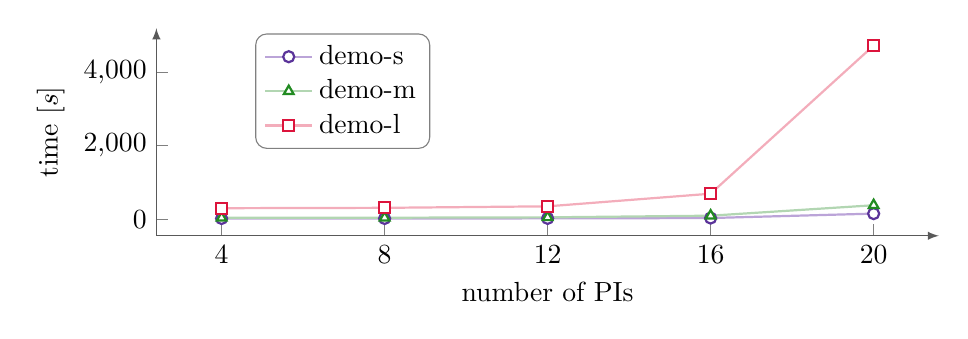
\begin{tikzpicture}
	\begin{axis}
	[legend style={at={(0.35,0.975)}, legend cell align={left}, anchor=north east, draw=gray, rounded corners}, height=12em, width=0.95\linewidth, axis y line*=left, axis x line*=bottom, axis line style={Black!65, -latex}, xlabel={number of PIs}, ylabel={time [$s$]}, xtick={4,8,12,16,20}]
	\addplot[RoyalPurple!35, thick, mark = *, mark options={solid, RoyalPurple, fill=white}, thick] coordinates {(4,17.399) (8,18.129) (12,20.27) (16,29.674) (20,149.757)};
	\addplot[ForestGreen!35, thick, mark = triangle*, mark options={solid, ForestGreen, fill=white}, thick] coordinates {(4,35.489) (8,38.726) (12,48.274) (16,93.432) (20,377.8)};
	\addplot[Crimson!35, thick, mark = square*, mark options={solid, Crimson, fill=white}, thick] coordinates {(4,297.485) (8,307.439) (12,348.038) (16,691.854) (20,4724.334)};
	\legend{demo-s, demo-m, demo-l} 
	\end{axis}
	\end{tikzpicture}
	\caption{\esp execution times on applications reported in Table~\ref{tab:expUseCase}.}
	\label{fig:espTime}
\end{figure}


\subsection{Framing Effort in the ESP}
\label{sec:time}
%\changeda{In section 7.4 you estimate how much time would be used by developers for annotations. I am not sure if you have the data on how much time was actually spent? If so, adding them would help strengthen your argumentation (although you claim that they would be substantially reduced with more experience) since we know what you base your estimates on.}
As mentioned in Section~\ref{sec:external_expert_design}, all framing tasks, including the annotation of the assets in the source code, were performed before the external industrial experts got involved in the assessment of the ESP. This enabled them to focus on the qualitative assessment without wasting their precious time on the more mechanistic framing tasks. This section analyzes the effort that is needed to perform those framing tasks with the ESP.

First, the user needs to annotate the assets in the source code. The ESP supports two options: manually annotating the source code or manually tagging code and data elements in the \esp. Our experiments only used source code annotations, which consist of (mostly single-line) pragmas and attributes~\cite{D5.11,D5.13} that identify the assets and specify security requirements. For users proficient with their syntax, typing out the annotations requires at most tens of seconds per asset.  

More time is required to determine precisely which elements in the source code need to be annotated because they correspond to the application assets. Security architects and software designers describe assets abstractly. When those are known upfront, developers can annotate their code as they write it, thus only requiring the aforementioned tens of seconds per asset. 
For developers that are familiar with the code base but need to annotate the code afterwards, we estimate that locating the assets in the code takes less than a minute for assets with high locality (e.g., single variables or single functions) to potentially tens of minutes for assets that are spread out more throughout the code base (e.g., the invocations of a specific reaction mechanism spread throughout the code for remote attestation).

The annotations were added to the ASPIRE use cases by their original developers after the development was finished. It was the first time they were adding our style of annotations. They hence faced a learning curve. Moreover, while adding the annotations, they had to validate the syntax and expressiveness of the annotation language on the fly. Had they already been proficient with the annotations beforehand and had they just needed to inject them without having to validate their design, we estimate that the time needed to annotate their use cases would have been less than one hour for the use cases with 25 assets, and less than two hours for the one with 43 assets.

In any case, locating the assets in the code base given abstract descriptions is something that any user of any non-trivial \softprot tool needs to do, both to configure the tool to protect the relevant code and to validate that that code has actually been protected by the tool. 
So compared to other \softprot approaches, the mentioned times are not considered overhead required to use the ESP. 
%
The same holds for selecting the attacks the user wants to mitigate and for determining which of the available {\softprot}s to consider. In the ESP, selecting attacks and {\softprot}s from the ones modelled in the KB happens with a click-of-a-button GUI interface. The time required for clicking is negligible compared to the time for deciding which ones to include or exclude. That decision making needs to happen with any decision support tool, so the ESP is not less efficient in this regard than any other decision making process. 
This discussion completes the answer to RQ1.d.1.


\subsection{Threats to Validity}
%\changeda{R1: As already stated, I would also recommend that you have all discussions related to validity in the same section, in this case moving the discussion of validity in section 6.5 to section 7.5. Also, as already stated, please explain better why the ESP limitations are primarily related to external validity (if you still think this is the case), as I would think they may relate also to other validity concerns. If you still want to keep the text in 6.5 (which I strongly advice against), please improve readability by giving the reader a short repetition of what the "ESP limitation discussed in Section 6.5) is - it is frustrating to have to go back and check if you forgot. (For the same reason, I would suggest that you also repeat the RQs when you first mention them in Section 7.)}

%\changeda{R1: In section 7.5, you explain your evaluation as "experiment" although you have not done an experiment (as far as I understand)}
We have checked our \changed{evaluation procedure} against a checklist of the possible threats to validity: construct, internal, conclusion, and external validity threats~\cite{wohlin00}, as well as instantiation validity threats~\cite{lukyanenko2014instantiation}.
	
%\changeda{R1: When it comes to construct validity, you do not cover risks related to your metrics not being the right ones for your RQs. This should be added. } 
Threats to \emph{construct validity} concern the metrics defined for the experiment.
We have used a set of standard metrics from the ISO. \changed{Nonetheless, the risk remains that the selected metrics are not the best ones for our assessment.} The evaluation scores were positive, negative, and partial, which appeared expressive enough for our purposes. However, we could not objectively assess these criteria' satisfaction as the questionnaires included open answers. 
To limit subjectivity, we have evaluated the answers within the ASPIRE project. Moreover, the ASPIRE project reviewers hired by the European Commission did not contradict our conclusions.
 
%%%% INTERNAL 
Threats to \emph{internal validity} concern the inferences between independent variables and experiment outcomes.
\changed{One possible noise factor that may confound the inference relates to the task comprehension. We assess this factor as negligible in this case.}
The task, resembling their day-to-day job and their typical applications, was described by the experts as clear; the use of the tool was documented; moreover, the experts were assisted in case of doubts (by their colleagues or by us). 
\changed{Another potential noise factor is the experts' commitment to do their tasks diligently before answering the questionnaire.}
We gave the experts the tool and the reports to be assessed offline. 
We hence cannot establish the effort they invested in using and reading them. 
We checked that all relevant artifacts were analysed in their comments (main attack paths and all the combinations of protections); however, we cannot assess their commitment accurately.
\changed{Moreover, another confounding factor is the actual objective evaluation.
The experts were selected from the industrial partners of the project. Even if they were asked to evaluate the artifact objectively, their judgment may have been biased by the will not to hinder the project and the positive evaluation by the European funding agency.}

%%%% EXTERNAL
%\changeda{R1: When it comes to external validity, I do not agree with your statement that "most of the external validity threats do not apply". You may have mitigated some of them by using practitioners etc, but this is no guarantee that the results of the evaluation apply to other experts developing other applications in other companies. } \\
%\abnote{from 6.5}\changeda{R1: As already stated, I would also recommend that you have all discussions related to validity in the same section, in this case moving the discussion of validity in section 6.5 to section 7.5. Also, as already stated, please explain better why the ESP limitations are primarily related to external validity (if you still think this is the case), as I would think they may relate also to other validity concerns. If you still want to keep the text in 6.5 (which I strongly advice against), please improve readability by giving the reader a short repetition of what the "ESP limitation discussed in Section 6.5) is - it is frustrating to have to go back and check if you forgot. (For the same reason, I would suggest that you also repeat the RQs when you first mention them in Section 7.)}
Threats to \emph{external validity} affect the generalisation of the research results to the real world, \ie experts who want to protect real applications using an automated decision support system.
\changed{In our case, the subjects of the evaluation are real experts that are protecting apps. The evaluation could hence be generalized to experts with a similar background protecting programs analogous to the ones presented in the evaluation and not too dissimilar from the ones they protect during normal job tasks in the same companies.
However, it does not necessarily extend to other experts protecting different applications in other companies.
Significant effort was invested in the use case applications to ensure that they are representative (in terms of size and complexity) of the code bases such experts have to protect in their daily jobs. However, since every expert only evaluated the \esp on one application, we cannot be sure that applications with different structures or from a different domain would yield similar results.}

\changed{Another potential threat to external validity concerns the possibility to generalize the evaluation made on a specific tool, the \esp, to general \softprot tasks, which may affect answers to RQ3.
In this case, we assessed this threat as negligible. Having automated a specific \softprot task, we have proved that automation is feasible, even if the same task could be done in different, possibly better ways. Moreover, the external experts performing the evaluation did not assess the ESP within the ASPIRE scope and requirements, as they did not know about the ASPIRE-defined scope. Instead, they evaluated it vis-à-vis their day-to-day job requirements. 
%
The limitations identified in Section~\ref{sec:coverage} on the \esp, which does not automate all tasks, do not apply, as RQ3 is related to individual parts of a risk management approach for \softprot.
% Therefore, our evaluation can answer RQ3, on the parts of the decision support that can be already automated, in general, and not on the \esp instance only despite not having automated all the identified constructs.
}

%\abnote{your argumentations on the RQ3, where written before we changed the RQ3. They answer the original question: is it possible to automate decision support (Boolean answer)? The current formulation of the question is: can we automate some tasks? Therefore these answers become a little bit overkill... I preferred leaving them in section 6.5.} {\color{orange}
% Moreover, the \esp limitation does not affect the possibility to generalize the case of the \esp and the tasks it automates to the possibility of performing \softprot tasks with an automated decision support tool.
% Indeed, all the activities that we have not (yet) automated can be performed manually. Existing methods to link technical threats and constraints to business risks are available as discussed in Section~\ref{sec:req:prioritization}, if not automated then certainly relying on human judgments. Furthermore, providing support for considering multiple attack phases requires no fundamental changes to the used models and methods.
% Experts can manually deal with those \sdlc issues in case future research would fail to provide automated solutions. 
% Decision support for functional requirements is actually simpler than support for non-functional requirements: functional requirements are typically expressed as "some form of protection functionality X needs to be included." If anything, such functional requirements limit the search space that the \softprot optimization algorithms need to explore, rather than complicating it. 
% %
% Fourth, whereas Section~\ref{sec:motivation_formalization_automation} argued for maximal formalization and automation to minimize the potential reduction in precision that can stem from the subjective expert judgments, within the ASPIRE project complete automation was not considered viable yet. Hence, the involvement of experts in making judgments was still accepted. So some aspects were not formalized and automated but instead left to human experts. This is the case for methods \methodlab{18} and \methodlab{132} for validating that the \softprot deployment is in line with made choices and requirements; for constructs \constructlab{5}, \constructlab{15}, and \constructlab{16} that serve to identify which application parts require protection despite not being primary assets; for identifying the path of least resistance (\constructlab{43}) among the enumerated attack paths; and for iterative mitigation decision making (\constructlab{50}, \methodlab{21}). An expert can use the \esp manually in an iterative manner, but the \esp does not automate this. Finally, while the \softprot tool developed in ASPIRE considers profile information for minimizing the performance impact of injected control flow obfuscations, the \esp does not consider profile information (\constructlab{35}) for selecting {\softprot}s. It is hence left up to the human expert to manually exclude expensive {\softprot}s for assets on which they cannot be afforded.
% %
% Fifth, the one remaining unsupported artifact is that of cookbooks with \softprot recipes (\methodlab{25}). Those cookbooks are only intended as backups for when automated \softprot selection is not supported. They are hence superfluous in the \esp.
%




%%%% CONCLUSION
%\changeda{R1: Some of the text related to conclusion validity seem to me to be as much related to internal validity (e.g., bias resulting from project-internal experts.} \abnote{moved to external validity}
Threats to \emph{conclusion validity} affect the validity of the methods to draw conclusions from the assessment.
In this case, we have asked experts to answer open questions from a standard questionnaire structured according to the main protection workflow. Given the experts' limited availability, a state-of-the-art controlled experiment was impossible. 
The main concern for our assessment is related to the limited number of experts involved, which does not allow us to use standard statistical methods.  


%\changeda{R1: The last two paragraphs concerning threats to validity should be moved to Section 7.5, so that the reader knows where to find discussions related to validity concerns. I am also not convinced that what you are talking about here is external validity. To me, it seems more related to instantiation validity - a type of validity very relevant for design science research (see e.g. Lukyanenko et al, 2014, "Instantiation Validity in IS Design Research"). I also wonder if it primarily has an impact on your answer to RQ3 (see also my comment on RQ3 and how you describe that you answer it in the introduction)}\bdsnote{I agree we should move the paragraphs, and I agree that discussing instantiation validity is something we should definitely do. Whether or not what I discuss below is instantiation validity or external validity, I am not sure ... }.

%%%% INSTANTIATION 
%\abnote{add instantiation validity here}

\changed{Finally, threats to \emph{instantiation validity} affect the possibility of considering the artifact we have implemented, i.e., the \esp, an instance of the theoretical object we had in mind, i.e., a semi-automated decision support system for \softprot \cite{instantiation-validity}.
The instantiation space is very large, as one can imagine many ways to implement all the tasks the \esp performs. In this space, we opted for a NIST-based four-phases approach. We have not considered alternative approaches, first and foremost because we were convinced upfront that the standard approach that works for other fields is also valid for \softprot. %\bdsnote{Where is the second?}
Secondly, we have implemented the \esp in the ASPIRE project, where resources for PoC and completion times were constrained. This relates to another threat, the artifact cost, that prevented the implementation of more alternatives.

Two more threats to instantiation validity apply to the \esp: auxiliary features and emergent properties, which stress the complexity of IT tools and oblige considering additional aspects that are not the main focus of the instantiation.
Indeed, the integration of the components and the definition of the workflow has revealed several auxiliary features related to the UI comprehension, the user experience, and the effectiveness of the designed workflow to cope with daily \softprot experts' tasks. 
Furthermore, several emergent properties appeared related to the complexity of the data, their relationships, and the correct data presentation. %\bdsnote{"to emerge" is basically the same as "to appear", so the wording in the previous sentence is strange.}
We tried to mitigate these threats by continuously interacting with the internal experts during the design, development, integration, and validation of the \esp and the data artifact it produces. Moreover, every time we received suggestions in the answers to the questionnaires, we have incorporated them before the next evaluation phase. Nonetheless, we cannot exclude that these threats to the instantiation validity may have an impact.}
%\bdsnote{In the above, I have replaced "We have managed them and try to reduce these threats" by "We tried to mitigate these threats". "We have managed them and ..." sounded too much like "We took care, so no worries anymore, and on to the next thing ..."}



}
	\caption{\label{fig:workflow}Schema of reinforcement learning in gray-box MDPs}
\end{figure}
